\documentclass[11pt,aspectratio=1610,xcolor=dvipsnames]{beamer}

\usetheme[
    background=light,
    numbering=fraction,
    block=fill,
    progressbar=frametitle
]{metropolis}

\usepackage{physics}
\usepackage{bbm}
\usepackage[most]{tcolorbox}
\usepackage{tikz}
\usetikzlibrary{arrows}
% \colorlet{LightLavender}{Lavender!40!}
\newtcolorbox{prob}{colback=red!5!white,colframe=red!75!black}
\usefonttheme[onlymath]{serif}
\usepackage{quantikz}

\newcommand{\R}{\mathbb{R}}
\newcommand{\U}[1]{\mathsf{U}(#1)}
\newcommand{\defeq}{\stackrel{\text{\tiny def}}{=}}


\newcommand{\problemstatement}{Hello}
\title{BQSKit}
\subtitle{An overview}
\date{Aug 31, 2022}
\author{Nate Stemen}
\institute{Unitary Fund}


\begin{document}

\maketitle

\begin{frame}{Overview}
	\begin{figure}[h]
		\centering
		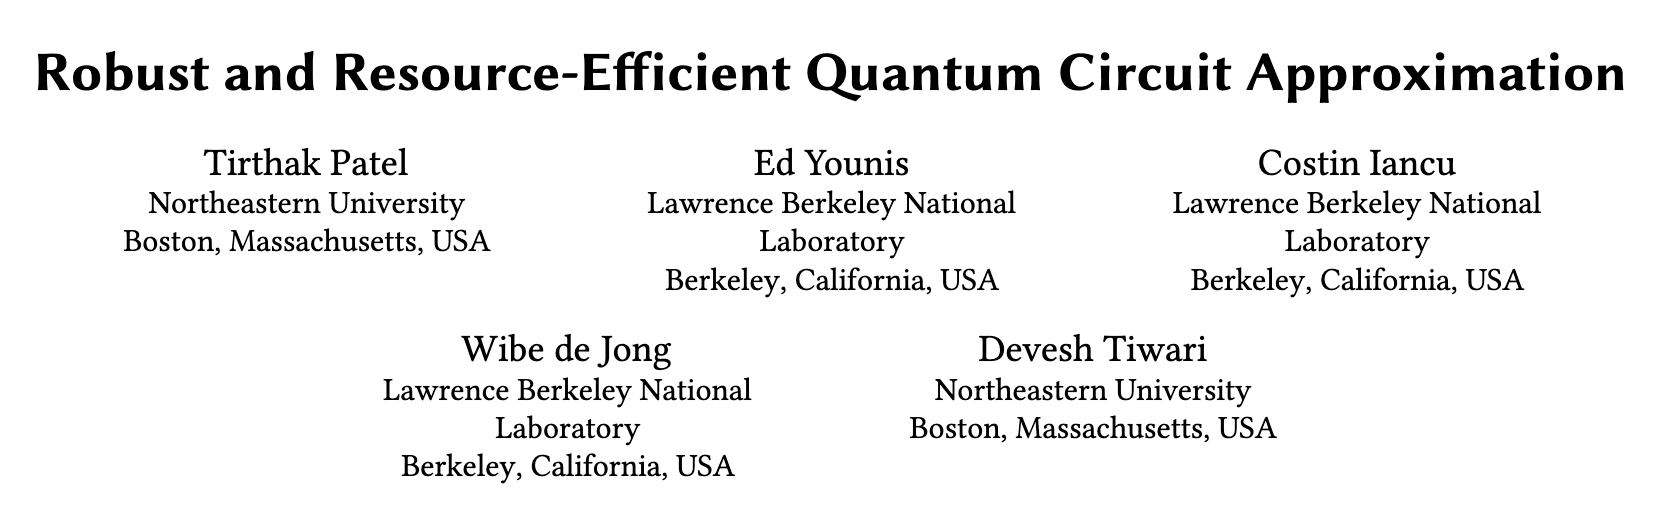
\includegraphics[width=\textwidth]{paper.png}
	\end{figure}
	\begin{center}
		\url{https://arxiv.org/abs/2108.12714}
	\end{center}
\end{frame}

\begin{frame}{Berkeley Quantum Synthesis Toolkit}
	\begin{quote}
		The Berkeley Quantum Synthesis Toolkit (BQSKit) is a superoptimizing quantum compiler and research vehicle that combines ideas from several projects at LBNL into an easily accessible and quickly extensible software suite.
	\end{quote}
\end{frame}

\begin{frame}{Berkeley Quantum Synthesis Toolkit}
	\begin{quote}
		The Berkeley Quantum Synthesis Toolkit (BQSKit) is a \textbf{superoptimizing} quantum \textbf{compiler} and research vehicle that combines ideas from several projects at LBNL into an easily accessible and quickly extensible software suite.
	\end{quote}
\end{frame}

\begin{frame}{What is a compiler?}
	\begin{figure}[h]
		\centering
		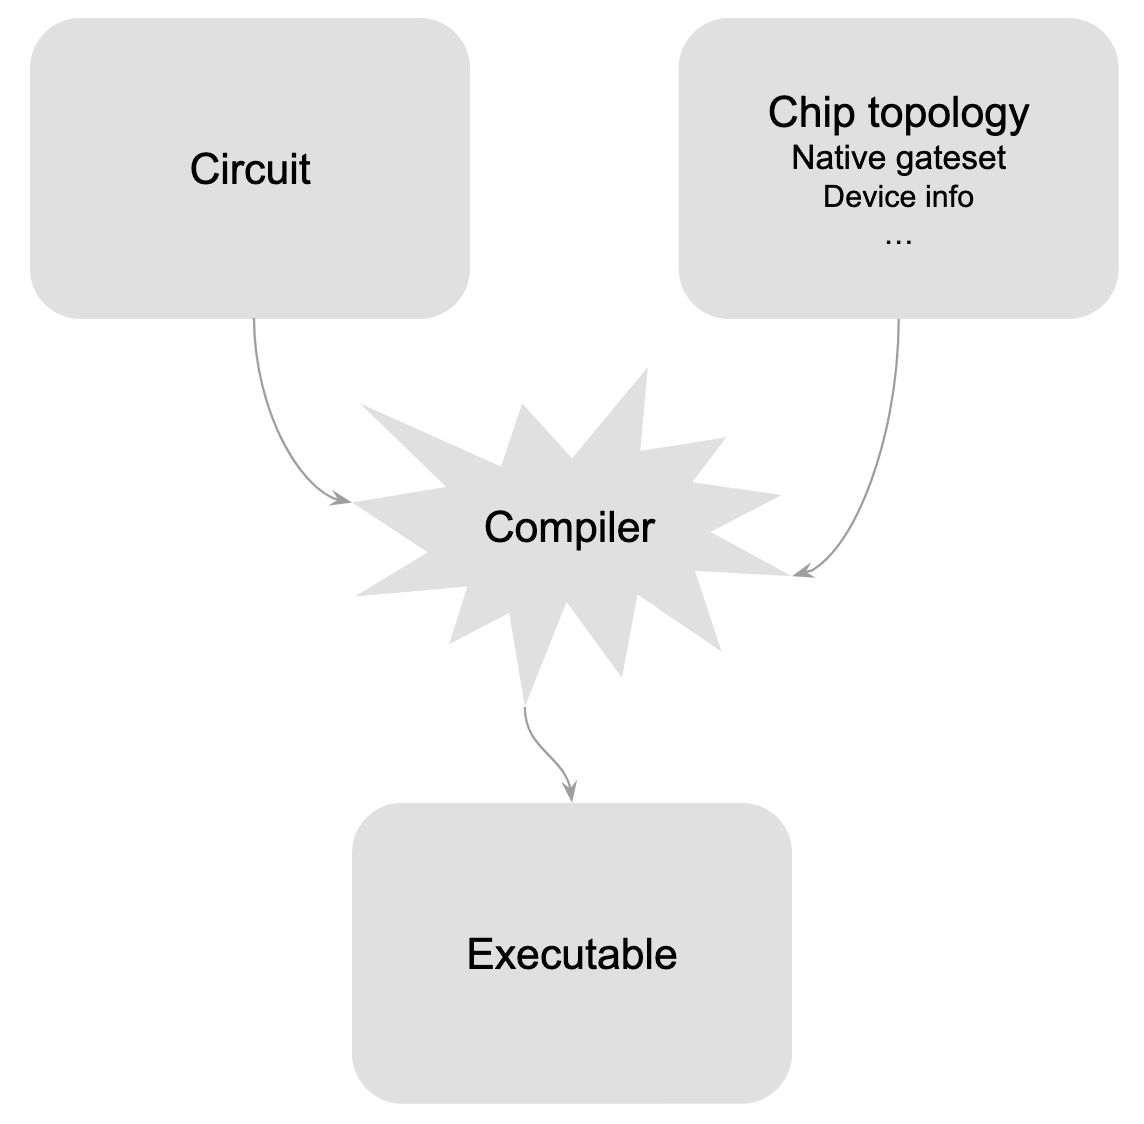
\includegraphics[width=0.6\textwidth]{compiler.png}
	\end{figure}
	% \begin{quantikz}
	% 	\lstick{$\ket{0}$} & \gate{H} & \ctrl{1} & \gate{U_1}   & \ctrl{1}   & \swap{2} & \ctrl{1}  & \qw \\
	% 	\lstick{$\ket{0}$} & \gate{H} & \targ{}  & \octrl{-1}   & \control{} & \qw      & \octrl{1} & \qw \\
	% 	&          &          &            &            &\targX{}  & \gate{U_2}  & \qw
	% \end{quantikz}
\end{frame}

\begin{frame}{What is ``superoptimizing''?}
	\begin{figure}[h]
		\centering
		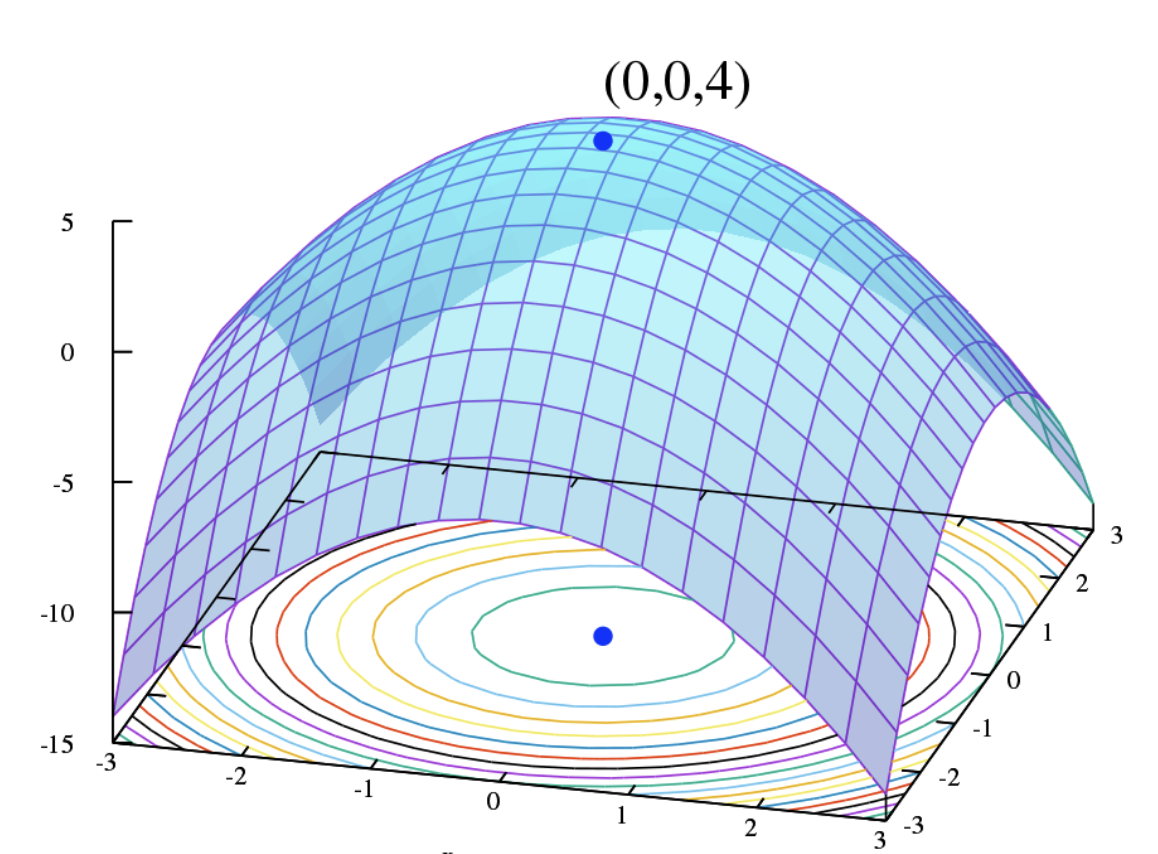
\includegraphics[width=0.6\textwidth]{optim.png}
	\end{figure}
\end{frame}

\begin{frame}{What is ``superoptimizing''?}
	\begin{figure}[h]
		\centering
		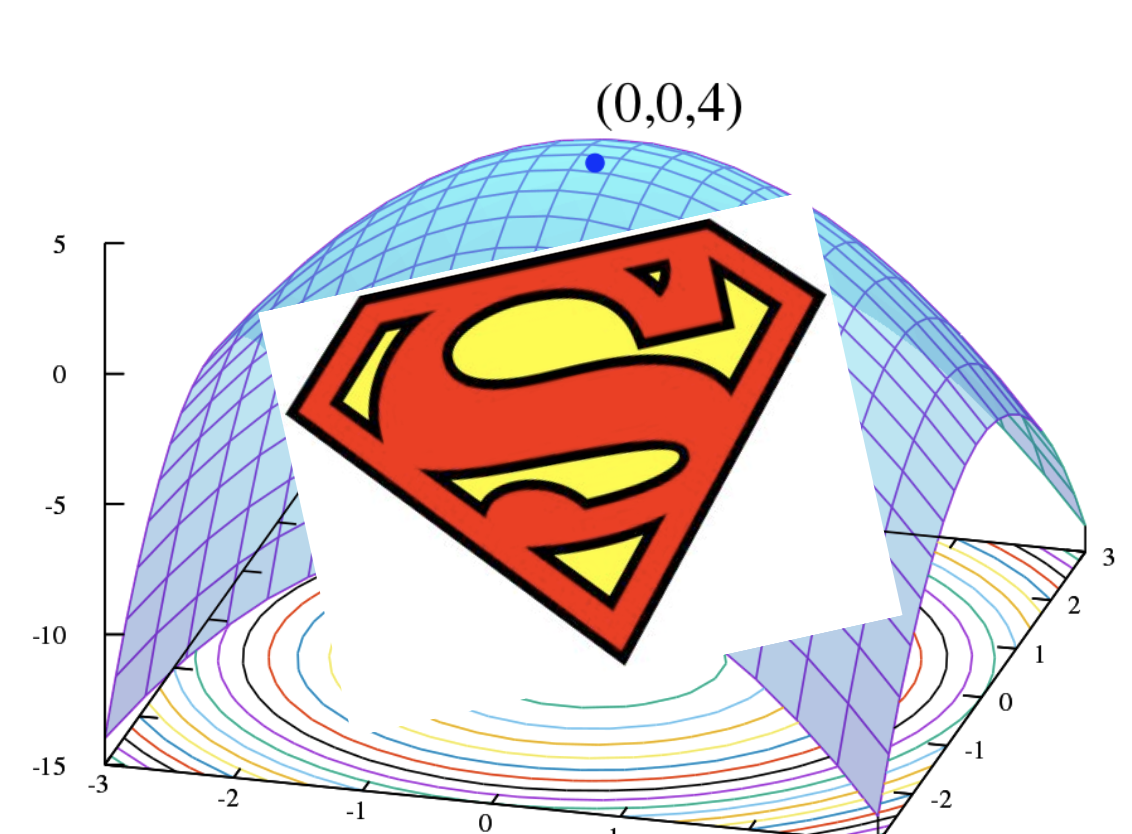
\includegraphics[width=0.6\textwidth]{super-optim.png}
	\end{figure}
\end{frame}

\begin{frame}{What does Qiskit do?}
	\begin{figure}[h]
		\centering
		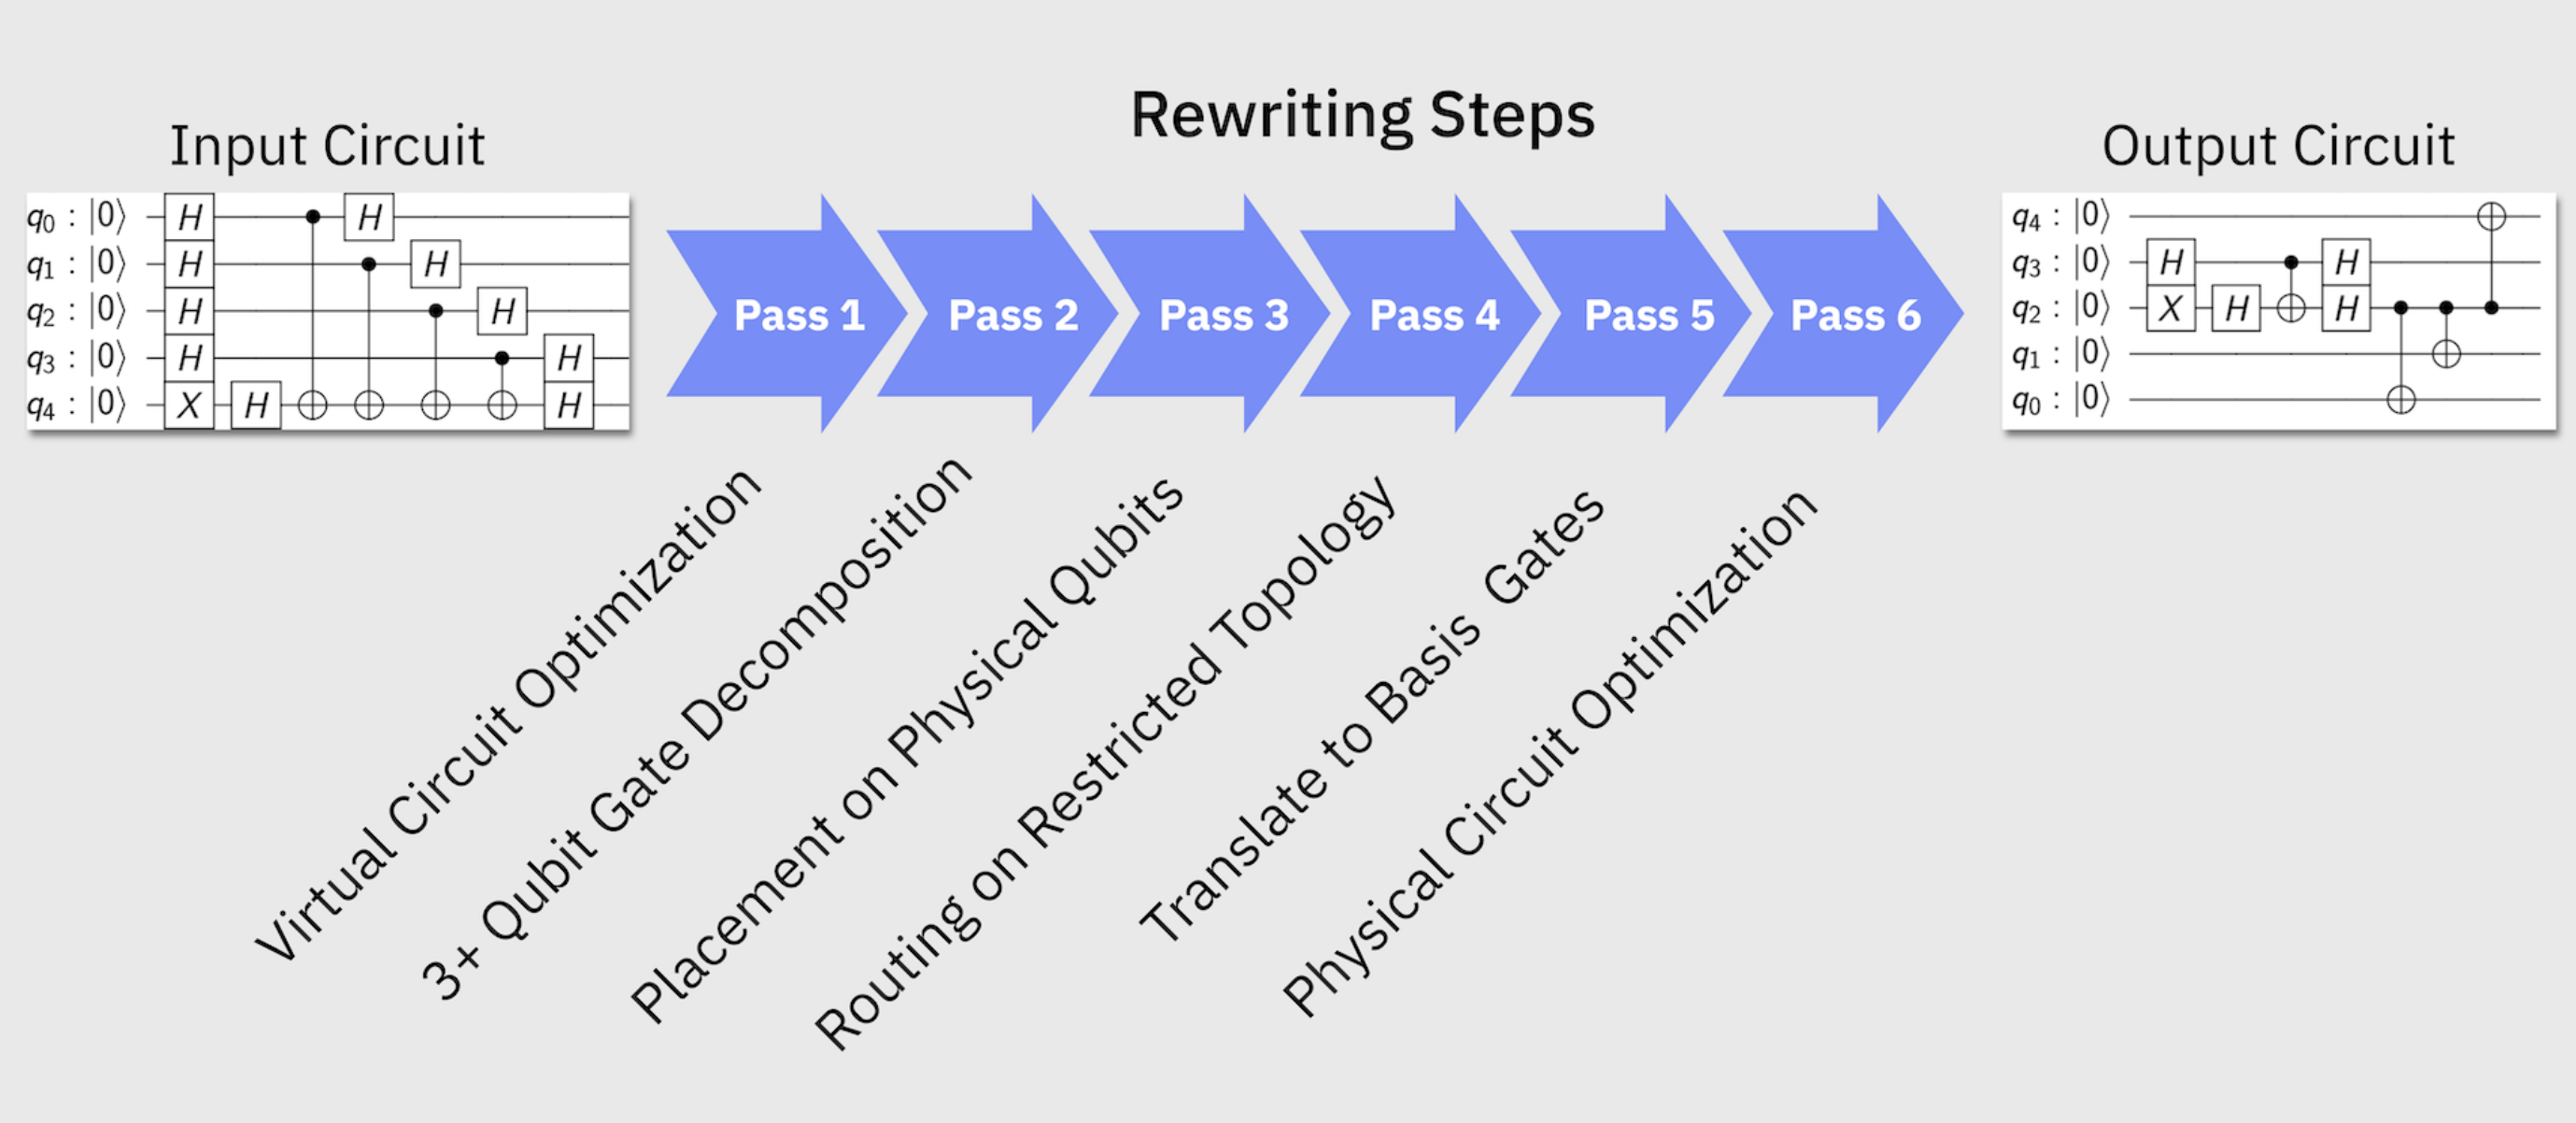
\includegraphics[width=0.9\textwidth]{qiskit.png}
	\end{figure}
\end{frame}

\begin{frame}{Unitary Synthesis}
	\begin{alertblock}{Problem Statement}
		Let $G$ be a gate set (i.e.\ a finite collection of unitary operators), and $U \in \U{2^n}$ be the \textbf{target unitary}.
		Find a sequence of gates $g_i \in G$ such that the target unitary $U$ can be written as $U = g_n \cdot g_{n - 1} \cdots g_2 \cdot g_1$.
	\end{alertblock}
	\begin{itemize}
		\item Need ways to ``compare'' the similarities of unitaries
		\item Hilbert-Schmidt inner product: $\langle U, V \rangle \defeq \tr(UV^\dagger)$
		\item Can turn this into a normalized distance function as $d_\text{HS}(U, V) \defeq \sqrt{1 - \frac{\abs{\langle U, V \rangle}}{2^{2n}}}$
		\item Total Variation Distance of probability distributions: $\frac{1}{2}\sum_{k = 1}{2^n}\abs{p_1(k) - p_2(k)}$
		      \begin{itemize}
			      \item $p_1(k)$ is probability of state $k$ after target unitary
			      \item $p_2(k)$ is probability of state $k$ after synthesized unitary
		      \end{itemize}
		\item $d_\text{HS}$ scales poorly due to unitaries growing exponential with number of qubits
	\end{itemize}
\end{frame}

\begin{frame}{Partitioning}
	\begin{center}
		\begin{quantikz}
			& \gate{}  & \ctrl{1} & \gate{}   & \targ{}   & \ctrl{1} & \targ{}   & \gate{}  & \gate{}   & \gate{}  & \qw \\
			& \ctrl{1} & \targ{}  & \gate{}   & \ctrl{-1} & \targ{}  & \ctrl{-1} & \gate{}  & \gate{}   & \ctrl{1} & \qw \\
			& \targ{}  & \gate{}  & \targ{}   & \gate{}   & \ctrl{1} & \targ{}   & \ctrl{1} & \targ{}   & \targ{}  & \qw \\
			& \gate{}  & \gate{}  & \ctrl{-1} & \gate{}   & \targ{}  & \ctrl{-1} & \targ{}  & \ctrl{-1} & \gate{} & \qw
		\end{quantikz}
	\end{center}
\end{frame}

\begin{frame}{Partitioning}
	\begin{center}
		\begin{quantikz}
			& \gate{}  & \ctrl{1} & \gate{}   & \targ{}   & \ctrl{1} & \targ{}   & \gate{}  & \gate{}   & \gate{}  & \qw \\
			& \ctrl{1} & \targ{}  & \gate{}   & \ctrl{-1} & \targ{}  & \ctrl{-1} & \gate{}  & \gate{}   & \ctrl{1} & \qw \\
			& \targ{}  & \gate{}  & \targ{}   & \gate{}   & \ctrl{1} & \targ{}   & \ctrl{1} & \targ{}   & \targ{}  & \qw \\
			& \gate{}  & \gate{}  & \ctrl{-1} & \gate{}   & \targ{}  & \ctrl{-1} & \targ{}  & \ctrl{-1} & \gate{} & \qw
		\end{quantikz}
		=
		\begin{quantikz}
			& \gate[3][1.2cm]{A} & \qw                & \qw \\
			&                    & \gate[3][1.2cm]{B} & \qw \\
			&                    &                    & \qw \\
			& \qw                &                    & \qw
		\end{quantikz}
	\end{center}
\end{frame}

\begin{frame}{Approximate block synthesis}
	\begin{columns}
		\column{0.5\textwidth}
		\centering
		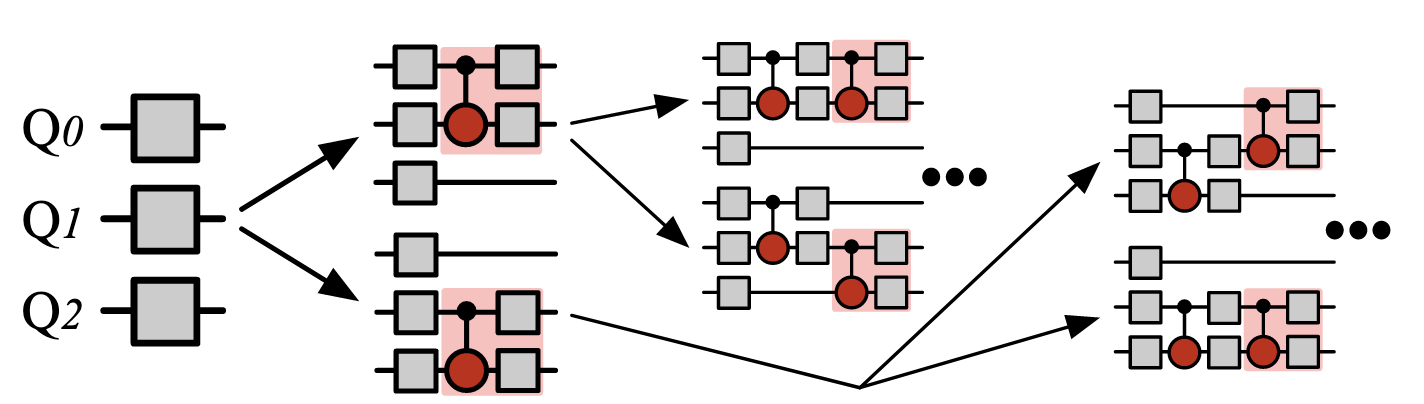
\includegraphics[width=\textwidth]{leap.png}
		\column{0.5\textwidth}
		\begin{itemize}
			\item Bottom up approach to synthesis
			\item Each layer consists of one $\mathsf{CNOT}$, and two single-qubit rotations
			\item Tree is pruned every few layers for branch with best approximations to target unitary
		\end{itemize}
	\end{columns}
\end{frame}

\begin{frame}{Block stitching}
	\begin{itemize}
		\item Synthesizing many, low-$\mathsf{CNOT}$ count circuits is easier than a single, but much more accurate one
		\item Averaging over multiple approximations can give an accurate representation of target unitary
		\item Dual annealing optimization: $\min f = (\mathsf{CNOT} \text{ count} + \text{dissamilarity})/2$
		\item $d_\text{HS}(U, V) \leq \sum_{k = 1}^K \varepsilon_k$ for $V$ being a partioned version of $U$ with $K$ blocks
	\end{itemize}
\end{frame}

\begin{frame}{Summary}
	\begin{itemize}
		\item BQSKit/QEST is a compiler primarily focused on reducing circuit depth via $\mathsf{CNOT}$ gate count reduction
		\item 30--80\% $\mathsf{CNOT}$ gate count reduction on ideal systems
	\end{itemize}
	\begin{columns}
		\column{0.5\textwidth}
		\begin{figure}[h]
			\centering
			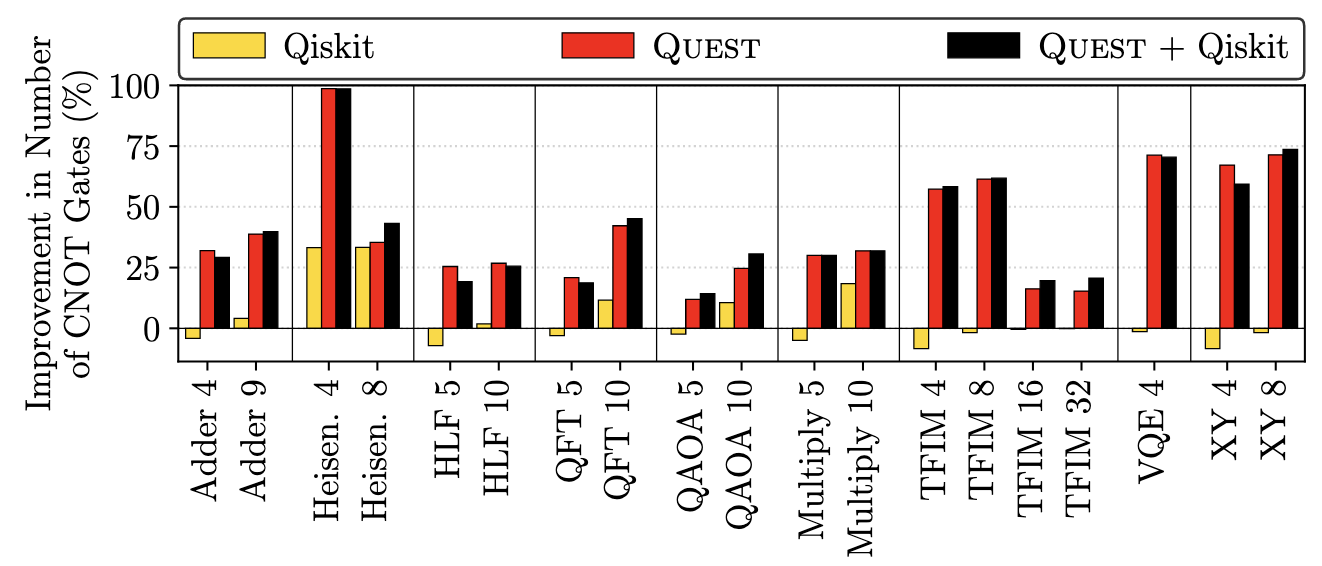
\includegraphics[width=\textwidth]{reductions.png}
		\end{figure}
		\column{0.5\textwidth}
		\begin{figure}[h]
			\centering
			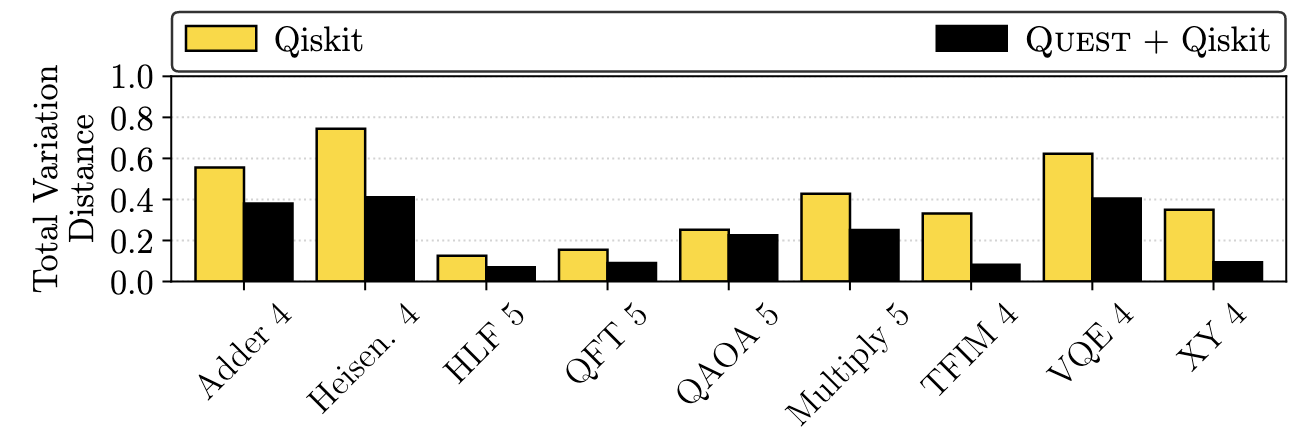
\includegraphics[width=\textwidth]{tvd-reductions.png}
		\end{figure}
	\end{columns}
\end{frame}

\end{document}
